\chapter{YPC的功能模块}

YPC在可信域和不可信域均有重要的功能和协议设计。本章试图模块化地抽象YPC,找出各组件之间的联系和依赖关系。从这些依赖关系中,找出与TEE各功能的对应关系,进而得出YPC对于TEE的依赖情况。

\begin{figure}
    \centering
    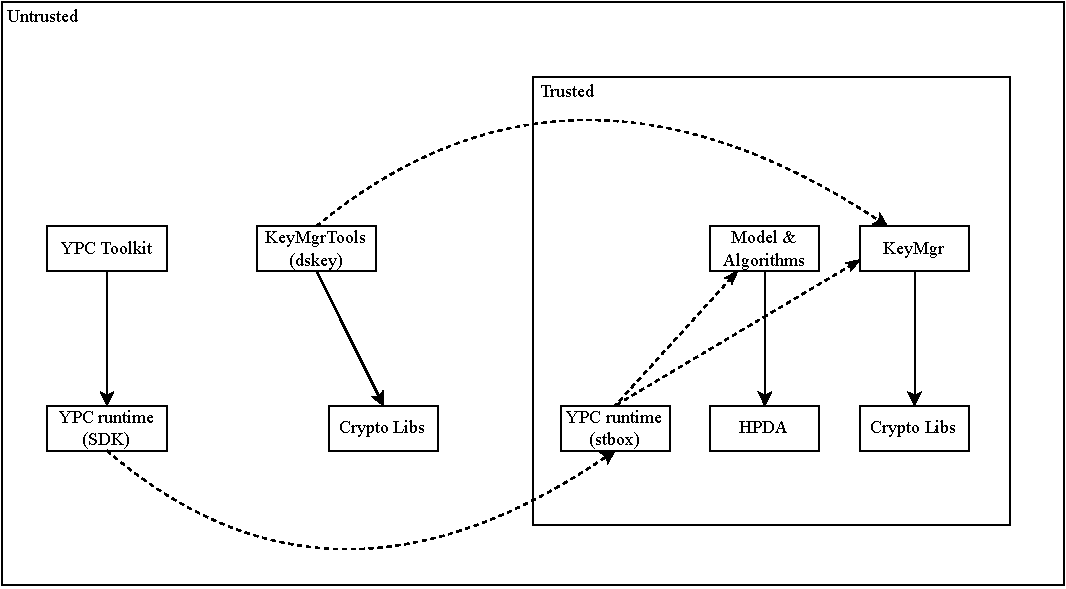
\includegraphics[width=140mm]{figure/ypc-modular.pdf}
    \caption{YPC模块关系图。整个系统分为两个区域,二者信任模型不同:其中Trusted为可信域,在TEE中存储和执行;Untrusted为不可信域,在TEE外执行。两个区域各有运行时(runtime)用于同步数据和系统状态。}
    \label{fig:ypc-modular}
\end{figure}

图\ref{fig:ypc-modular}展示了YPC的模块化框图。在初始化阶段,运行在非可信域中的KeyMgrTools将由EK加密后的平台相关密钥信息,通过可信信道传输到可信域中的KeyMgr中。

$S^D_c = seal_{EK}(S^D_p)$

$S^D_p = unseal_{EK}(S^D_c)$

从协议角度,YPC的简化模型包括四个角色,
\begin{enumerate}
    \item 数据提供方(data provider)\\ 
    提供任务图中的原始数据,以自己持有的枢公钥加密原始数据。
    \item (算法)模型提供方(model provider)\\ 
    开发者,算法提供方也可以提供相应的模型。
    \item 数据使用方(data user)\\ 
    得到最终的计算任务输出。
    \item 算力提供方,又称计算平台(computing platform)\\ 
    安装Fidelius隐私计算节点,持有典公钥。
\end{enumerate}

YPC支持的机密计算功能和特性包括,本地数据可用不可见、托管数据可用不可见、结果的可信性证明、结果不可见、数据用途限制、模型不可见、模型用途限制、任务参数不可见、原子交付。

本文描述YPC部分特性的实现方法,并以伪代码形式展示。

\begin{enumerate}
    \item 本地数据可用不可见\\
    本地数据可通过加密后存储到外设上。

    \begin{lstlisting}
bytes local_data; 
bytes encrypted_data = encrypt(local_data, 
    platform_pkey);
t_mem_wr(epc_addr, 
    local_data, local_data.length); 
    \end{lstlisting}

    \item 托管数据可用不可见\\
    将数据加密后,托管到第三方存储。

    \begin{lstlisting}
bytes local_data; 
bytes encrypted_data = encrypt(local_data, dest_pkey); 
// upload to delegatee storages
        
// download from delegatee storages
bytes delegated_data; 
bytes dest_pk; 
t_mem_wr(dpk_epc_addr, 
    dest_pk, dest_pk.length); 
t_mem_wr(dd_epc_addr, 
    delegated_data, delegated_data.length);   
    \end{lstlisting}

    \item 结果的可信性证明\\ 
    计算平台得到计算结果后,通过$S^D$对结果签名,保证计算结果的正确性完整性。

    \begin{lstlisting}
// Executed in TEE
Report report; 
report = local_attest(model_einfo); 
// send report to keymgr enclave
    \end{lstlisting}

    \item 结果不可见\\ 
    计算平台得到计算结果后,将结果加密后,返回数据使用方。

    \begin{lstlisting}
// Executed in TEE
bytes result; 
bytes encrypted_result = encrypt(result, du_pkey); 
    \end{lstlisting}

    \item 数据用途限制\\ 
    (还未实现)计算平台解析元数据,检查数据用途。
    \begin{lstlisting}
// Check params in model enclave
    \end{lstlisting}
    \item 模型不可见\\ 
    模型源代码不可见,仅将编译后的二进制文件传入计算平台。

\begin{lstlisting}
// Signed dynamic library

// Possible implementations in the future: 
bytes model_so; 
bytes encrypted_model = encrypt(model_so, platform_pkey); 
\end{lstlisting}

    \item 模型用途限制\\ 
    计算平台解析模型元数据,检查模型参数和用途。
    \item 任务参数不可见\\ 
    数据使用方将计算任务参数加密后,传入计算平台。
    \item 原子交付\\
    通过智能合约,保证任务结果交付和任务费用交付的原子性绑定。
\end{enumerate}

